\documentclass[11pt]{article}

\usepackage[margin=1in]{geometry}
\usepackage[T1]{fontenc}
\usepackage[utf8]{inputenc}
\usepackage{lmodern}
\usepackage{microtype}
\usepackage{amsmath,amssymb,amsthm,mathtools}
\usepackage{bm}
\usepackage{booktabs,array,longtable}
\usepackage{xcolor}
\usepackage{hyperref}
\usepackage[most]{tcolorbox}
\usepackage{tikz}
\usepackage{pgfplots}
\usepackage{tikz-3dplot}
\usepackage{enumitem}
\usepackage{caption}
\usepackage{float}
\usepackage{fancyhdr}
\usepackage{titlesec}

\pgfplotsset{compat=1.18}
\usepgfplotslibrary{fillbetween}
\usetikzlibrary{arrows.meta,calc,intersections,patterns,decorations.pathreplacing,positioning,3d,backgrounds,shadings}

\hypersetup{
  colorlinks=true,
  linkcolor=blue!60!black,
  urlcolor=blue!60!black,
  citecolor=blue!60!black,
  pdftitle={Chapter 13. Double Integrals and Riemann Sums}
}

\setlength{\headheight}{14pt}
\setlength{\parindent}{0pt}
\setlength{\parskip}{0.65em}
\setlist[itemize]{topsep=2pt,itemsep=2pt}
\setlist[enumerate]{topsep=2pt,itemsep=2pt}

\titleformat{\section}{\large\bfseries}{\thesection}{0.6em}{}
\titleformat{\subsection}{\normalsize\bfseries}{\thesubsection}{0.6em}{}

\pagestyle{fancy}
\fancyhf{}
\lhead{Chapter 13. Double Integrals and Riemann Sums}
\rhead{\thepage}
\renewcommand{\headrulewidth}{0.4pt}

\newtcolorbox{chaptergoalbox}{
  enhanced,
  colback=blue!4,
  colframe=blue!55!black,
  boxrule=0.8pt,
  arc=2mm,
  left=2mm,right=2mm,top=1.5mm,bottom=1.5mm
}

\newtcolorbox{goalbox}{
  enhanced,
  colback=green!4,
  colframe=green!45!black,
  title=Learning objectives,
  fonttitle=\bfseries,
  boxrule=0.7pt,
  arc=2mm
}

\newtcolorbox{notebox}[1][]{
  enhanced,
  breakable,
  colback=blue!3,
  colframe=blue!50!black,
  fonttitle=\bfseries,
  title=#1,
  boxrule=0.7pt,
  arc=2mm
}

\newtcolorbox{importantbox}[1][]{
  enhanced,
  breakable,
  colback=red!3,
  colframe=red!60!black,
  fonttitle=\bfseries,
  title=#1,
  boxrule=0.7pt,
  arc=2mm
}

\newtcolorbox{tipbox}[1][]{
  enhanced,
  breakable,
  colback=green!3,
  colframe=green!45!black,
  fonttitle=\bfseries,
  title=#1,
  boxrule=0.7pt,
  arc=2mm
}

\newtcolorbox{warningbox}[1][]{
  enhanced,
  breakable,
  colback=yellow!8,
  colframe=orange!80!black,
  fonttitle=\bfseries,
  title=#1,
  boxrule=0.7pt,
  arc=2mm
}

\newtcbtheorem[number within=section]{examplebox}{Example}{
  enhanced,
  breakable,
  colback=white,
  colframe=blue!60!black,
  colbacktitle=blue!60!black,
  fonttitle=\bfseries,
  boxrule=0.7pt,
  arc=1.5mm,
  left=2mm,right=2mm,top=1mm,bottom=1mm
}{ex}

\newcommand{\R}{\mathbb R}
\newcommand{\dA}{\,dA}
\newcommand{\dd}{\,d}
\newcommand{\Area}{\operatorname{Area}}
\newcommand{\E}{\mathbb E}

\begin{document}

\begin{center}
  {\LARGE\bfseries Chapter 13. Double Integrals and Riemann Sums\par}
  \vspace{0.3em}
  {\large Area accumulation, volume, numerical approximation, and iterated integration\par}
\end{center}

\begin{chaptergoalbox}
\textbf{Chapter goal.} A single integral adds small contributions along a line. A double integral adds small contributions over a two-dimensional region. This chapter develops double integrals from Riemann sums, explains their geometric meaning, and shows how Fubini's theorem turns a two-dimensional accumulation problem into two ordinary one-variable integrations.

The ideas in this chapter are important bridges from calculus to applied mathematics, statistics, data science, and machine learning. A double integral may represent volume, mass, charge, expected value, average temperature, total risk, probability over a region, or total loss accumulated over a two-parameter domain.
\[
\text{total amount}\approx \sum \text{value at a sample point}\times \text{small area}.
\]
When the rectangles become very small, the approximation becomes an integral.
\end{chaptergoalbox}

\begin{goalbox}
After studying this chapter, you should be able to:
\begin{enumerate}
  \item explain a double integral as the limit of double Riemann sums;
  \item compute area elements $dA=\Delta x\Delta y$ on rectangular partitions;
  \item interpret $\iint_R f(x,y)\dA$ as volume when $f\ge 0$;
  \item interpret double integrals as signed accumulation when $f$ changes sign;
  \item approximate double integrals using sample points and the midpoint rule;
  \item evaluate double integrals over rectangles using Fubini's theorem;
  \item compute average values over rectangles;
  \item connect double integrals to density, mass, numerical integration, and probability.
\end{enumerate}
\end{goalbox}

\section{From one-dimensional area to two-dimensional accumulation}

Recall the definite integral of a continuous function $f(x)$ on an interval $[a,b]$:
\[
\int_a^b f(x)\dd x=\lim_{\Delta x\to 0}\sum_i f(x_i^*)\Delta x.
\]
Geometrically, if $f(x)\ge 0$, this is the area under the curve $y=f(x)$ above the interval $[a,b]$. Computationally, it means:
\begin{enumerate}
  \item divide the interval into small subintervals;
  \item choose a sample point in each subinterval;
  \item multiply height by width;
  \item add the pieces;
  \item pass to the limit.
\end{enumerate}

A double integral follows the same pattern, but the base region is two-dimensional. Instead of small intervals, we use small rectangles. Instead of length $\Delta x$, each small piece has area
\[
\Delta A=\Delta x\Delta y.
\]
If the height above $(x,y)$ is $f(x,y)$, then a small rectangular column has approximate volume
\[
f(x_{ij}^*,y_{ij}^*)\Delta A.
\]
Adding all such columns gives a double Riemann sum.

\begin{figure}[H]
\centering
\begin{minipage}{0.48\textwidth}
\centering
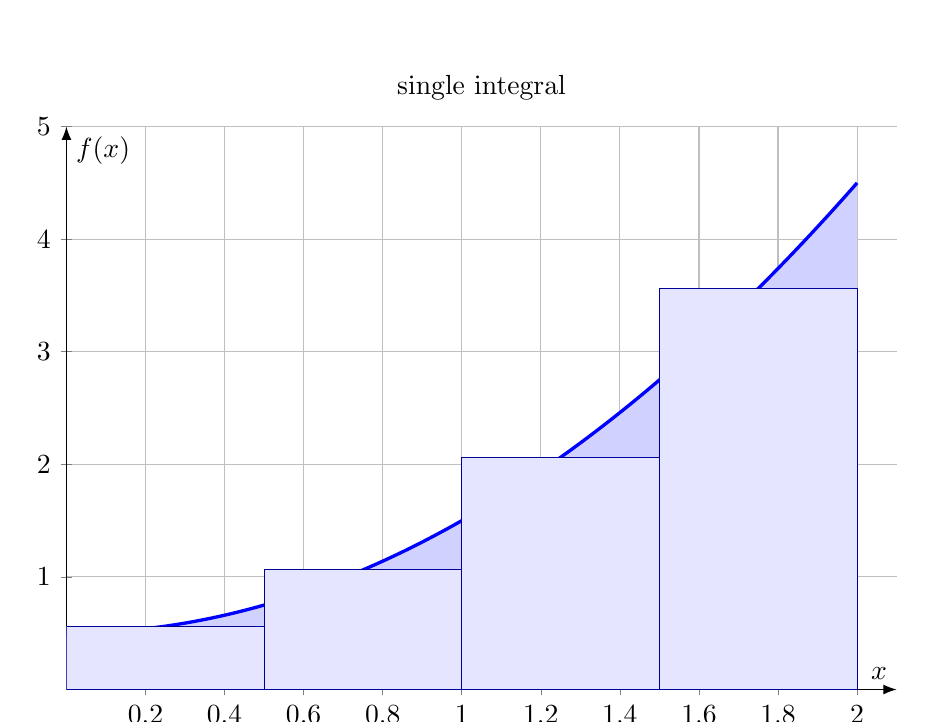
\begin{tikzpicture}
\begin{axis}[
  width=\textwidth,height=0.72\textwidth,
  xmin=0,xmax=2.1,ymin=0,ymax=5,
  axis lines=middle,
  xlabel={$x$},ylabel={$f(x)$},
  grid=both,
  title={single integral},
  axis line style={-Latex}
]
\addplot[name path=curve,domain=0:2,samples=150,very thick,blue] {x^2+0.5};
\path[name path=axisline] (axis cs:0,0)--(axis cs:2,0);
\addplot[blue!18] fill between[of=curve and axisline];
\foreach \x in {0.25,0.75,1.25,1.75}{
  \pgfmathsetmacro{\height}{\x*\x+0.5}
  \addplot[draw=blue!60!black,fill=blue!10] coordinates {(\x-0.25,0) (\x+0.25,0) (\x+0.25,\height) (\x-0.25,\height) (\x-0.25,0)};
}
\end{axis}
\end{tikzpicture}
\end{minipage}\hfill
\begin{minipage}{0.48\textwidth}
\centering
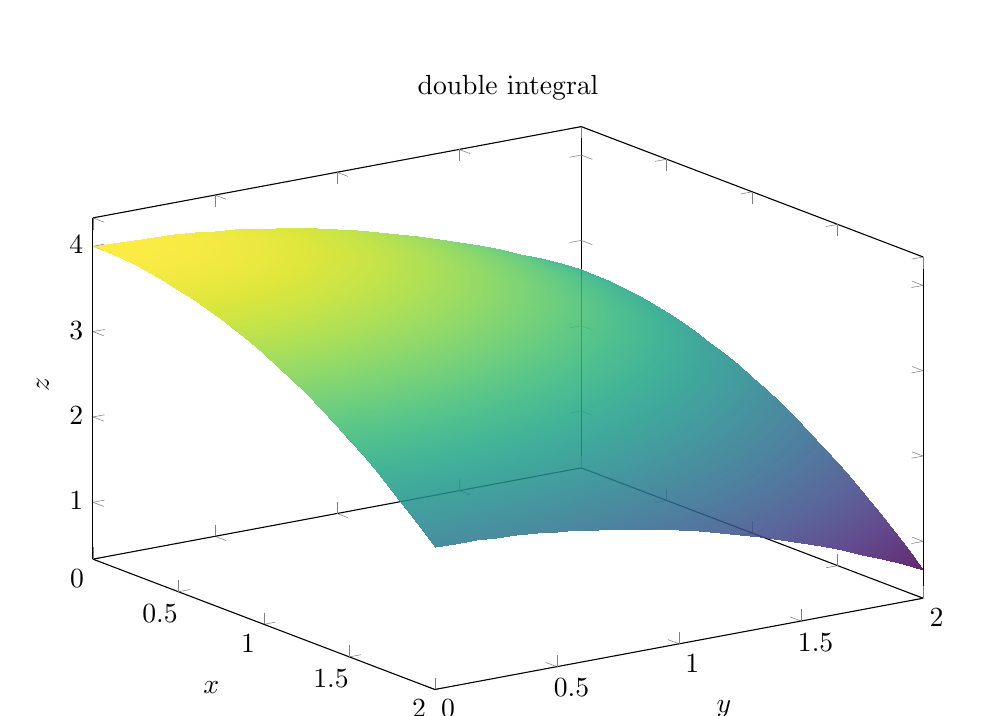
\begin{tikzpicture}
\begin{axis}[
  width=\textwidth,height=0.72\textwidth,
  view={55}{25},
  xlabel={$x$},ylabel={$y$},zlabel={$z$},
  domain=0:2,y domain=0:2,
  samples=25,samples y=25,
  colormap/viridis,
  title={double integral}
]
\addplot3[surf,shader=interp,opacity=0.85] {4 - x^2/2 - y^2/3};
\end{axis}
\end{tikzpicture}
\end{minipage}
\caption{A single integral accumulates over an interval; a double integral accumulates over a region.}
\end{figure}

\begin{notebox}[The main shift]
A single integral adds over a line-like set. A double integral adds over an area-like set. The algebra looks similar, but the geometry changes from intervals to regions and from rectangles to columns.
\end{notebox}

\section{Rectangular regions and partitions}

For the first part of the theory, we focus on a rectangular region
\[
R=[a,b]\times[c,d]=\{(x,y):a\le x\le b,\ c\le y\le d\}.
\]
Divide $[a,b]$ into $m$ equal subintervals and $[c,d]$ into $n$ equal subintervals. Then
\[
\Delta x=\frac{b-a}{m},\qquad \Delta y=\frac{d-c}{n},\qquad \Delta A=\Delta x\Delta y.
\]
This divides $R$ into $mn$ small rectangles $R_{ij}$. In each $R_{ij}$, choose a sample point $(x_{ij}^*,y_{ij}^*)$. The associated double Riemann sum is
\[
\sum_{i=1}^m\sum_{j=1}^n f(x_{ij}^*,y_{ij}^*)\Delta A.
\]
If $f(x,y)\ge 0$, this sum estimates the volume under $z=f(x,y)$ and above $R$.

\begin{figure}[H]
\centering
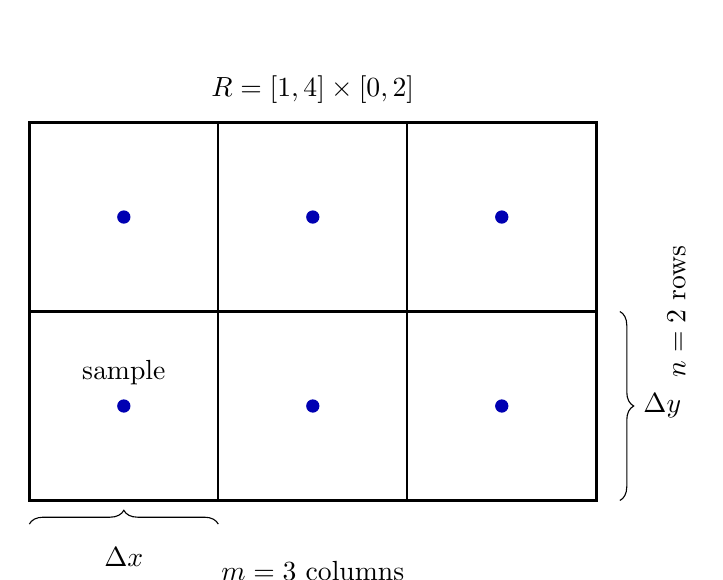
\begin{tikzpicture}[scale=1.2]
  \draw[very thick] (0,0) rectangle (6,4);
  \foreach \x in {2,4}{\draw[thick] (\x,0)--(\x,4);}
  \draw[thick] (0,2)--(6,2);
  \foreach \x in {1,3,5}{\foreach \y in {1,3}{\fill[blue!70!black] (\x,\y) circle (2pt);}}
  \draw[decorate,decoration={brace,amplitude=5pt}] (0,-0.25)--(2,-0.25) node[midway,below=5pt] {$\Delta x$};
  \draw[decorate,decoration={brace,amplitude=5pt,mirror}] (6.25,0)--(6.25,2) node[midway,right=5pt] {$\Delta y$};
  \node at (3,4.35) {$R=[1,4]\times[0,2]$};
  \node[fill=white,inner sep=1pt] at (1,1.35) {sample};
  \node at (3,-0.75) {$m=3$ columns};
  \node[rotate=90] at (6.85,2) {$n=2$ rows};
\end{tikzpicture}
\caption{A rectangle divided into subrectangles. Each subrectangle contributes one term to a double Riemann sum.}
\end{figure}

\section{The double integral on a rectangle}

Let $f$ be a function defined on a rectangle $R=[a,b]\times[c,d]$. If the double Riemann sums approach a single limiting value as the partition becomes finer, independent of the sample points, then $f$ is integrable on $R$. The limit is called the \emph{double integral} of $f$ over $R$.

\begin{importantbox}[Definition: double integral over a rectangle]
For a sufficiently nice function $f$ on $R$,
\[
\iint_R f(x,y)\dA=\lim_{m,n\to\infty}\sum_{i=1}^m\sum_{j=1}^n f(x_{ij}^*,y_{ij}^*)\Delta A.
\]
Here $dA$ represents a small piece of area. In rectangular coordinates, it is approximated by $\Delta A=\Delta x\Delta y$.
\end{importantbox}

The notation $dA$ reminds us that the integral is adding over area. Later, when we change coordinates, the expression for $dA$ will change. In rectangular coordinates,
\[
dA=dx\,dy\qquad \text{or}\qquad dA=dy\,dx.
\]

\subsection*{Volume interpretation}
If $f(x,y)\ge 0$ on $R$, then
\[
\iint_R f(x,y)\dA
\]
is the volume of the solid below the surface $z=f(x,y)$ and above the base region $R$.

\begin{figure}[H]
\centering
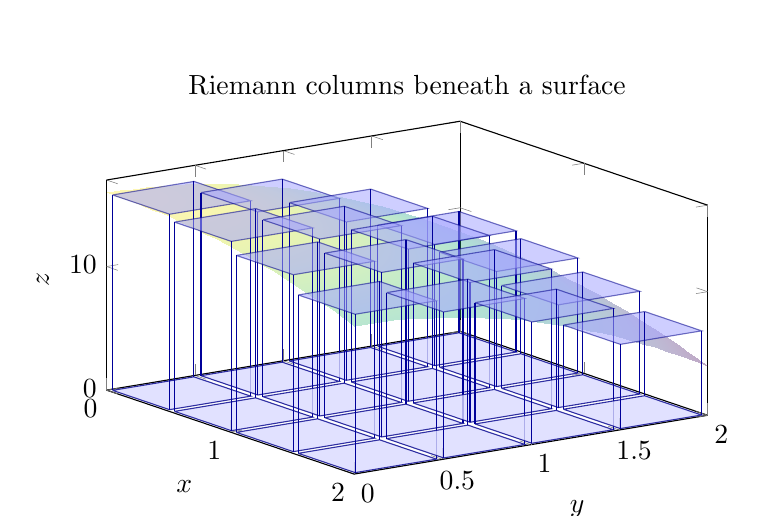
\begin{tikzpicture}
\begin{axis}[
  width=0.76\textwidth,height=0.50\textwidth,
  view={55}{26},
  xlabel={$x$},ylabel={$y$},zlabel={$z$},
  xmin=0,xmax=2,ymin=0,ymax=2,zmin=0,zmax=17,
  colormap/viridis,
  title={Riemann columns beneath a surface}
]
\addplot3[surf,domain=0:2,y domain=0:2,samples=28,samples y=28,shader=interp,opacity=0.35] {16 - x^2 - 2*y^2};
\foreach \i in {0.25,0.75,1.25,1.75}{
  \foreach \j in {0.25,0.75,1.25,1.75}{
    \pgfmathsetmacro{\h}{16-\i*\i-2*\j*\j}
    \addplot3[draw=blue!55!black,fill=blue!15,opacity=0.8] coordinates { (\i-0.23,\j-0.23,0) (\i+0.23,\j-0.23,0) (\i+0.23,\j+0.23,0) (\i-0.23,\j+0.23,0) (\i-0.23,\j-0.23,0) };
    \addplot3[draw=blue!55!black,fill=blue!35,opacity=0.55] coordinates { (\i-0.23,\j-0.23,\h) (\i+0.23,\j-0.23,\h) (\i+0.23,\j+0.23,\h) (\i-0.23,\j+0.23,\h) (\i-0.23,\j-0.23,\h) };
    \addplot3[blue!60!black] coordinates {(\i-0.23,\j-0.23,0) (\i-0.23,\j-0.23,\h)};
    \addplot3[blue!60!black] coordinates {(\i+0.23,\j-0.23,0) (\i+0.23,\j-0.23,\h)};
    \addplot3[blue!60!black] coordinates {(\i+0.23,\j+0.23,0) (\i+0.23,\j+0.23,\h)};
    \addplot3[blue!60!black] coordinates {(\i-0.23,\j+0.23,0) (\i-0.23,\j+0.23,\h)};
  }
}
\end{axis}
\end{tikzpicture}
\caption{A double Riemann sum approximates volume by rectangular columns beneath $z=16-x^2-2y^2$.}
\end{figure}

\section{Worked example: upper-right Riemann sum}

\begin{examplebox}{Upper-right sum for $f(x,y)=x^2y$}{upperright}
Consider
\[
f(x,y)=x^2y,\qquad R=[1,4]\times[0,2].
\]
Use $m=3$ subdivisions in the $x$-direction and $n=2$ subdivisions in the $y$-direction. Then
\[
\Delta x=\frac{4-1}{3}=1,\qquad \Delta y=\frac{2-0}{2}=1,\qquad \Delta A=1.
\]
Using upper-right corners as sample points gives
\[
x=2,3,4,\qquad y=1,2.
\]
Therefore
\[
\begin{aligned}
\sum_{i=1}^3\sum_{j=1}^2 f(x_i^*,y_j^*)\Delta A
&=f(2,1)+f(3,1)+f(4,1)+f(2,2)+f(3,2)+f(4,2)\\
&=4+9+16+8+18+32\\
&=87.
\end{aligned}
\]
Since $x^2y$ increases as $x$ and $y$ increase on this rectangle, upper-right corners overestimate the integral.
\end{examplebox}

\begin{center}
\begin{tabular}{@{}ccccc@{}}
\toprule
$x$ & $y$ & $f(x,y)=x^2y$ & $\Delta A$ & contribution \\
\midrule
2 & 1 & 4 & 1 & 4 \\
3 & 1 & 9 & 1 & 9 \\
4 & 1 & 16 & 1 & 16 \\
2 & 2 & 8 & 1 & 8 \\
3 & 2 & 18 & 1 & 18 \\
4 & 2 & 32 & 1 & 32 \\
\midrule
\multicolumn{4}{r}{Total} & 87 \\
\bottomrule
\end{tabular}
\end{center}

\section{The midpoint rule for double integrals}

The \emph{midpoint rule} uses the center of each subrectangle as the sample point. For a rectangle divided into $m$ by $n$ equal subrectangles,
\[
\iint_R f(x,y)\dA\approx \sum_{i=1}^m\sum_{j=1}^n f(\bar x_i,\bar y_j)\Delta A,
\]
where $\bar x_i$ and $\bar y_j$ are midpoint coordinates.

\begin{examplebox}{Midpoint rule for $x^2y$}{midpoint}
Again let
\[
f(x,y)=x^2y,\qquad R=[1,4]\times[0,2],\qquad m=3,\qquad n=2.
\]
The midpoint sample values are
\[
x=1.5,2.5,3.5,\qquad y=0.5,1.5.
\]
Thus
\[
\iint_R x^2y\dA\approx \sum_{x\in\{1.5,2.5,3.5\}}\sum_{y\in\{0.5,1.5\}}x^2y=44.5.
\]
The exact value, found later in this chapter, is $42$, so the midpoint estimate is much closer than the upper-right estimate $87$.
\end{examplebox}

\begin{figure}[H]
\centering
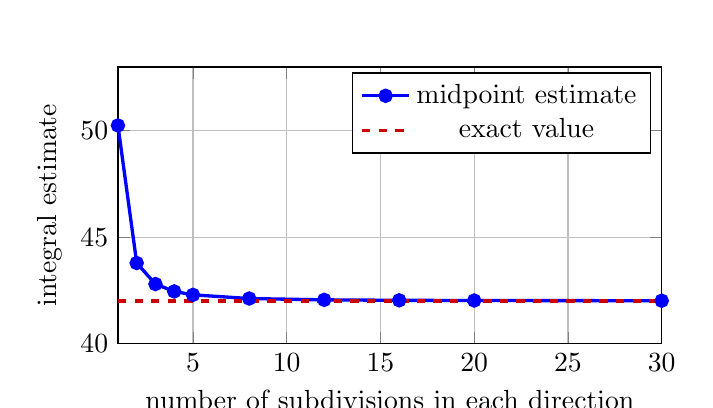
\begin{tikzpicture}
\begin{axis}[
  width=0.70\textwidth,height=0.42\textwidth,
  xmin=1,xmax=30,
  ymin=40,ymax=53,
  xlabel={number of subdivisions in each direction},
  ylabel={integral estimate},
  grid=both,
  legend style={at={(0.98,0.98)},anchor=north east,fill=white}
]
\addplot[very thick,blue,mark=*] coordinates {(1,50.25) (2,43.78125) (3,42.7917) (4,42.4453) (5,42.285) (8,42.1113) (12,42.0495) (16,42.0278) (20,42.0178) (30,42.0079)};
\addlegendentry{midpoint estimate}
\addplot[red!80!black,dashed,very thick] coordinates {(1,42) (30,42)};
\addlegendentry{exact value}
\end{axis}
\end{tikzpicture}
\caption{Midpoint Riemann sums converge to the exact double integral as the grid becomes finer.}
\end{figure}

\begin{tipbox}[Why midpoint sampling is often good]
The midpoint rule samples each rectangle at its center. For smooth functions, this often balances overestimates and underestimates better than using only corners. This is one reason midpoint-type ideas appear in numerical integration, finite-volume methods, and simulation.
\end{tipbox}

\section{Fubini's theorem on rectangles}

Riemann sums define the double integral, but limits of double sums are rarely the easiest way to compute exact answers. The key computational result is Fubini's theorem.

\begin{importantbox}[Fubini's theorem for rectangles]
If $f$ is continuous on $R=[a,b]\times[c,d]$, then
\[
\iint_R f(x,y)\dA=\int_a^b\int_c^d f(x,y)\dd y\dd x=\int_c^d\int_a^b f(x,y)\dd x\dd y.
\]
The double integral can be computed by integrating one variable at a time.
\end{importantbox}

The inner integral treats the other variable as constant. For example,
\[
\int_1^4 x^2y\dd x=y\int_1^4x^2\dd x=y\left[\frac{x^3}{3}\right]_1^4=21y.
\]
Then
\[
\int_0^2 21y\dd y=\left[\frac{21y^2}{2}\right]_0^2=42.
\]
Therefore
\[
\iint_{[1,4]\times[0,2]}x^2y\dA=42.
\]

The same answer is obtained in the other order:
\[
\int_1^4\int_0^2 x^2y\dd y\dd x=\int_1^4 2x^2\dd x=42.
\]
The order changes the intermediate expressions, but not the final value.

\begin{figure}[H]
\centering
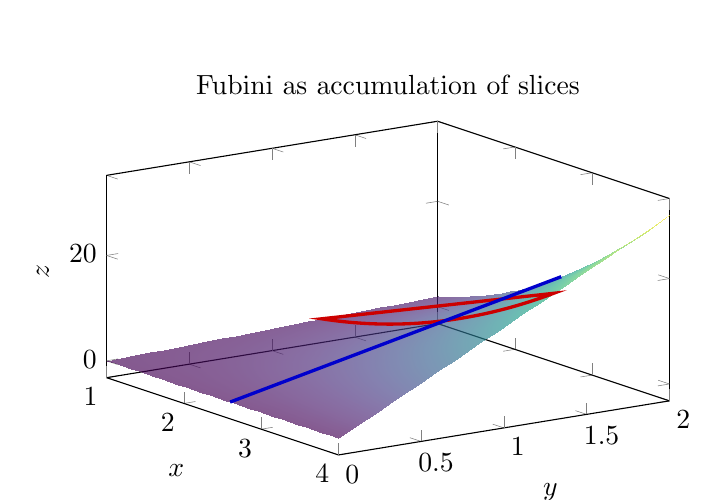
\begin{tikzpicture}
\begin{axis}[
  width=0.72\textwidth,height=0.48\textwidth,
  view={55}{25},
  xlabel={$x$},ylabel={$y$},zlabel={$z$},
  domain=1:4,y domain=0:2,
  samples=30,samples y=24,
  colormap/viridis,
  title={Fubini as accumulation of slices}
]
\addplot3[surf,shader=interp,opacity=0.65] {x^2*y};
\addplot3[very thick,red!80!black,domain=1:4,samples=150] ({x},{1.3},{x^2*1.3});
\addplot3[very thick,blue!80!black,domain=0:2,samples=150] ({2.6},{x},{2.6^2*x});
\end{axis}
\end{tikzpicture}
\caption{Fubini's theorem computes a double integral by accumulating one-dimensional slices of the surface.}
\end{figure}

\section{Separability and product structure}

Sometimes a function separates into a product of a function of $x$ and a function of $y$:
\[
f(x,y)=g(x)h(y).
\]
On a rectangle, Fubini's theorem gives
\[
\iint_{[a,b]\times[c,d]}g(x)h(y)\dA=\left(\int_a^b g(x)\dd x\right)\left(\int_c^d h(y)\dd y\right).
\]
For example,
\[
\iint_{[0,\pi]\times[0,1]}y\sin x\dA=\left(\int_0^\pi\sin x\dd x\right)\left(\int_0^1y\dd y\right)=2\cdot\frac12=1.
\]
This product structure appears frequently in probability. If two random variables are independent, their joint density often factors as $p(x,y)=p_X(x)p_Y(y)$.

\section{Signed accumulation}

If $f(x,y)$ takes both positive and negative values, then
\[
\iint_R f(x,y)\dA
\]
is no longer ordinary volume. It is \emph{signed volume}: positive parts above the $xy$-plane count positively, and negative parts below the $xy$-plane count negatively. For example, on a symmetric rectangle,
\[
\iint_{[-1,1]\times[0,2]}xy\dA=0,
\]
because the positive and negative contributions cancel.

\begin{figure}[H]
\centering
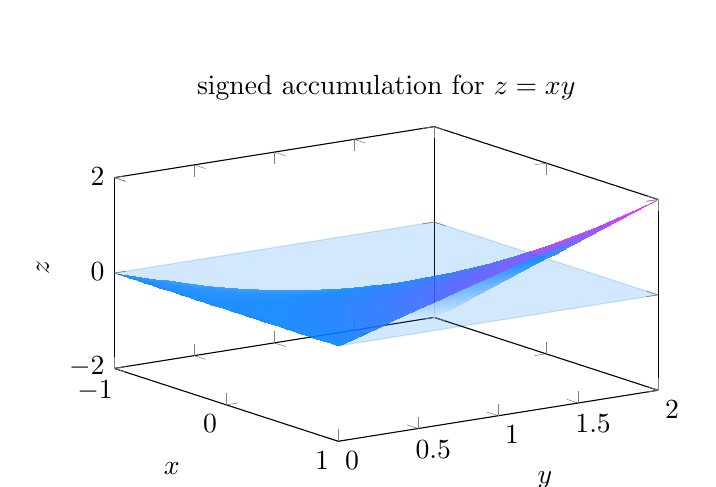
\begin{tikzpicture}
\begin{axis}[
  width=0.70\textwidth,height=0.46\textwidth,
  view={55}{25},
  xlabel={$x$},ylabel={$y$},zlabel={$z$},
  domain=-1:1,y domain=0:2,
  samples=31,samples y=25,
  colormap/cool,
  zmin=-2,zmax=2,
  title={signed accumulation for $z=xy$}
]
\addplot3[surf,shader=interp,opacity=0.85] {x*y};
\addplot3[surf,domain=-1:1,y domain=0:2,samples=2,samples y=2,opacity=0.18] {0};
\end{axis}
\end{tikzpicture}
\caption{A double integral can measure signed accumulation when the surface has positive and negative parts.}
\end{figure}

\begin{warningbox}[Volume versus signed volume]
If $f\ge 0$, the double integral is a volume. If $f$ changes sign, the double integral is signed volume. To compute total physical volume between the surface and the plane, one would integrate $|f(x,y)|$ instead.
\end{warningbox}

\section{Average value over a rectangle}

The average value of a one-variable function over $[a,b]$ is
\[
f_{\mathrm{avg}}=\frac{1}{b-a}\int_a^b f(x)\dd x.
\]
The average value of a two-variable function over a region $R$ is
\[
f_{\mathrm{avg}}=\frac{1}{\Area(R)}\iint_R f(x,y)\dA.
\]
For a rectangle $R=[a,b]\times[c,d]$,
\[
\Area(R)=(b-a)(d-c).
\]

\begin{examplebox}{Average height}{avgheight}
Let
\[
f(x,y)=16-x^2-2y^2,\qquad R=[0,2]\times[0,2].
\]
The double integral is
\[
\iint_R(16-x^2-2y^2)\dA=\int_0^2\int_0^2(16-x^2-2y^2)\dd y\dd x=\frac{136}{3}.
\]
Since $\Area(R)=4$, the average value is
\[
f_{\mathrm{avg}}=\frac14\cdot\frac{136}{3}=\frac{34}{3}.
\]
In a physical interpretation, this is the average height of the surface over the rectangular base.
\end{examplebox}

\begin{figure}[H]
\centering
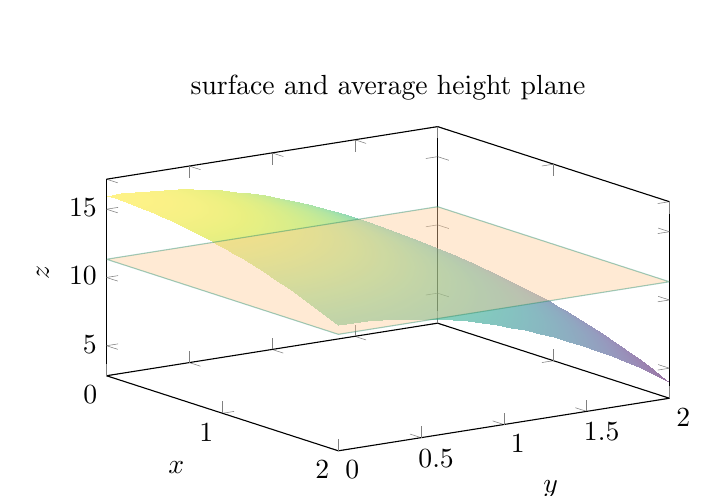
\begin{tikzpicture}
\begin{axis}[
  width=0.72\textwidth,height=0.47\textwidth,
  view={55}{25},
  xlabel={$x$},ylabel={$y$},zlabel={$z$},
  domain=0:2,y domain=0:2,
  samples=30,samples y=24,
  colormap/viridis,
  title={surface and average height plane}
]
\addplot3[surf,shader=interp,opacity=0.55] {16 - x^2 - 2*y^2};
\addplot3[surf,domain=0:2,y domain=0:2,samples=2,samples y=2,fill=orange!40,draw=orange!70!black,opacity=0.42] {34/3};
\end{axis}
\end{tikzpicture}
\caption{The average value is the constant height that gives the same total volume over the base region.}
\end{figure}

\section{Mass and density on a rectangular plate}

Suppose a thin rectangular plate occupies a region $R$ in the $xy$-plane. If its density at $(x,y)$ is $\rho(x,y)$, then the mass of a small rectangle is approximately
\[
\rho(x_{ij}^*,y_{ij}^*)\Delta A.
\]
The total mass is therefore
\[
M=\iint_R\rho(x,y)\dA.
\]

\begin{examplebox}{Mass of a rectangular plate}{densityplate}
Let
\[
\rho(x,y)=2+x+y,\qquad R=[0,3]\times[0,2].
\]
Then
\[
\begin{aligned}
M&=\int_0^3\int_0^2(2+x+y)\dd y\dd x\\
&=\int_0^3\left[2y+xy+\frac{y^2}{2}\right]_0^2\dd x\\
&=\int_0^3(6+2x)\dd x=27.
\end{aligned}
\]
The double integral is not just a geometric volume. It is a general accumulation tool: density times area gives mass, and the integral adds these contributions.
\end{examplebox}

\begin{figure}[H]
\centering
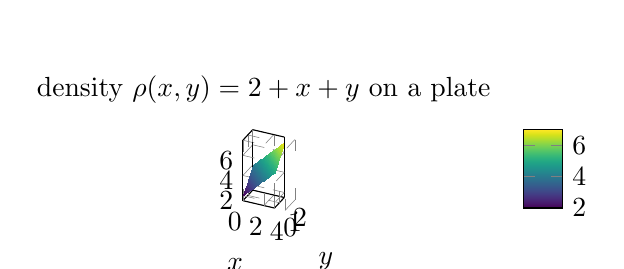
\begin{tikzpicture}
\begin{axis}[
  width=0.62\textwidth,height=0.43\textwidth,
  xmin=0,xmax=3,ymin=0,ymax=2,
  axis equal image,
  xlabel={$x$},ylabel={$y$},
  title={density $\rho(x,y)=2+x+y$ on a plate},
  colorbar,
  colormap/viridis
]
\addplot3[surf,shader=interp,domain=0:3,y domain=0:2,samples=30,samples y=20,view={0}{90}] {2+x+y};
\end{axis}
\end{tikzpicture}
\caption{A density field over a rectangular plate. Integrating density over area gives mass.}
\end{figure}

\section{Numerical double integration}

In applications, exact symbolic integration may not be available. A function may be known only through data, simulation, or a black-box model. Then Riemann sums become algorithms.

A reusable midpoint rule for rectangles has the form
\[
\text{estimate}=\sum_{i=1}^m\sum_{j=1}^n f(\bar x_i,\bar y_j)\Delta x\Delta y.
\]
For high-dimensional applied mathematics and machine learning, this point of view matters. Integrals are often approximated numerically, and sums over grids, samples, or data points are discrete versions of continuous accumulation.

\section{Monte Carlo viewpoint}

A double integral over a rectangle can also be estimated by random sampling. If $R$ has area $A$ and $(X,Y)$ is sampled uniformly from $R$, then
\[
\iint_R f(x,y)\dA=A\,\E[f(X,Y)].
\]
This gives the Monte Carlo estimator
\[
\iint_R f(x,y)\dA\approx A\cdot\frac1N\sum_{k=1}^N f(X_k,Y_k).
\]
Monte Carlo integration is usually less accurate than grid-based integration in low dimensions, but it becomes central in statistics, Bayesian computation, uncertainty quantification, and high-dimensional integration.

\begin{figure}[H]
\centering
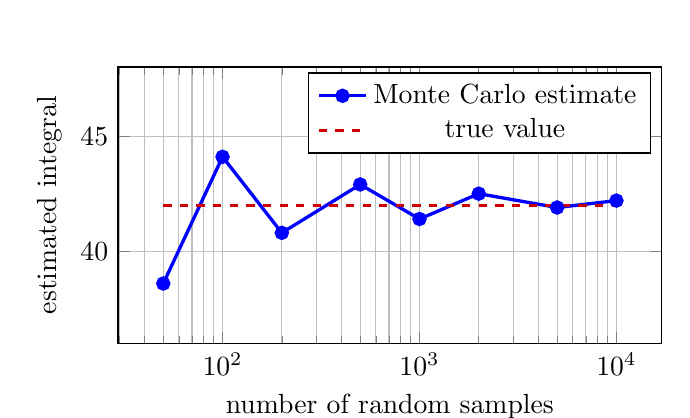
\begin{tikzpicture}
\begin{semilogxaxis}[
  width=0.70\textwidth,height=0.42\textwidth,
  xlabel={number of random samples},
  ylabel={estimated integral},
  grid=both,
  ymin=36,ymax=48,
  legend style={at={(0.98,0.98)},anchor=north east,fill=white}
]
\addplot[very thick,blue,mark=*] coordinates {(50,38.6) (100,44.1) (200,40.8) (500,42.9) (1000,41.4) (2000,42.5) (5000,41.9) (10000,42.2)};
\addlegendentry{Monte Carlo estimate}
\addplot[red!80!black,dashed,very thick] coordinates {(50,42) (10000,42)};
\addlegendentry{true value}
\end{semilogxaxis}
\end{tikzpicture}
\caption{Monte Carlo estimates fluctuate randomly but approach the true integral as the number of samples increases.}
\end{figure}

\section{Double integrals and probability on rectangles}

If $p(x,y)$ is a joint probability density on a region $R$, then probabilities are double integrals:
\[
P((X,Y)\in A)=\iint_A p(x,y)\dA.
\]
For a rectangular event $A=[a,b]\times[c,d]$, we compute
\[
P(a\le X\le b,\ c\le Y\le d)=\int_a^b\int_c^d p(x,y)\dd y\dd x.
\]
This is one reason double integrals are essential preparation for statistics. Later chapters will develop non-rectangular regions, change of variables, and multivariate normal densities in more detail.

\begin{figure}[H]
\centering
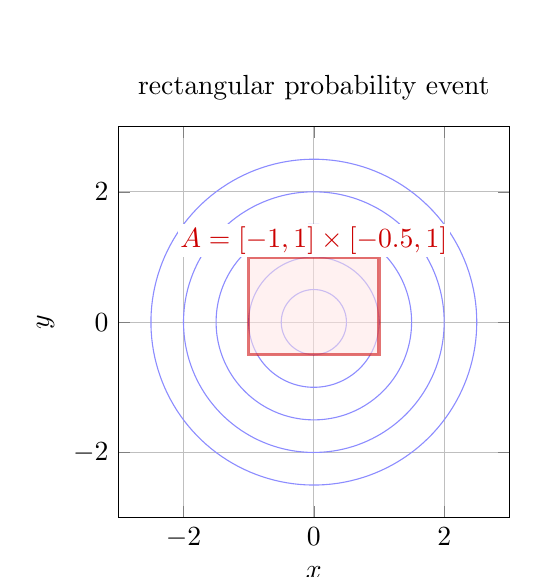
\begin{tikzpicture}
\begin{axis}[
  width=0.62\textwidth,height=0.54\textwidth,
  xmin=-3,xmax=3,ymin=-3,ymax=3,
  axis equal image,
  xlabel={$x$},ylabel={$y$},
  grid=both,
  title={rectangular probability event},
  axis line style={-Latex}
]
\foreach \r in {0.5,1,1.5,2,2.5}{\addplot[domain=0:360,samples=160,blue!45] ({\r*cos(x)},{\r*sin(x)});}
\draw[very thick,red!80!black,fill=red!10,opacity=0.55] (axis cs:-1,-0.5) rectangle (axis cs:1,1);
\node[red!80!black,fill=white,inner sep=1pt] at (axis cs:0,1.25) {$A=[-1,1]\times[-0.5,1]$};
\end{axis}
\end{tikzpicture}
\caption{Probability over a rectangle is the double integral of a density over that rectangle.}
\end{figure}

\section{Common mistakes}

\begin{warningbox}[Mistake 1: forgetting $\Delta A$]
A Riemann sum must have the form
\[
\sum f(x_{ij}^*,y_{ij}^*)\Delta A.
\]
The values of $f$ alone do not approximate an integral. They must be multiplied by area.
\end{warningbox}

\begin{warningbox}[Mistake 2: confusing the order of integration]
The expression
\[
\int_a^b\int_c^d f(x,y)\dd y\dd x
\]
means: integrate with respect to $y$ first, then integrate the resulting function of $x$ with respect to $x$.
\end{warningbox}

\begin{warningbox}[Mistake 3: assuming every double integral is volume]
A double integral is ordinary volume only when $f\ge 0$. Otherwise it is signed accumulation.
\end{warningbox}

\begin{warningbox}[Mistake 4: using Fubini without checking the region]
In this chapter, the main region is a rectangle. In the next chapter, we will study general regions where bounds may depend on variables.
\end{warningbox}

\section{Chapter exercises}

\subsection*{Conceptual problems}
\begin{enumerate}
  \item Explain in words why the term $f(x_{ij}^*,y_{ij}^*)\Delta A$ represents a small volume when $f\ge 0$.
  \item What is the difference between a double Riemann sum and a double integral?
  \item Why does $dA$ represent area rather than length?
  \item Explain why $\iint_R f(x,y)\dA$ may be negative if $f$ changes sign.
  \item Describe the difference between a midpoint estimate and an upper-right corner estimate.
\end{enumerate}

\subsection*{Computational problems}
\begin{enumerate}[start=6]
  \item Let $f(x,y)=3x+2y$ on $R=[0,2]\times[1,3]$. Use $m=2$, $n=2$, and upper-right sample points to approximate $\iint_R f\dA$.
  \item Repeat Problem 6 using midpoint sample points.
  \item Compute the exact value of $\iint_R(3x+2y)\dA$.
  \item Evaluate $\iint_{[0,1]\times[0,2]}xy^2\dA$.
  \item Evaluate $\iint_{[1,3]\times[0,\pi]}x\cos y\dA$.
  \item Evaluate $\iint_{[-1,1]\times[-1,1]}x^3y^2\dA$ without doing a long calculation. Explain the cancellation.
  \item Find the average value of $f(x,y)=x+y$ on $[0,4]\times[0,2]$.
  \item Find the mass of a rectangular plate $[0,2]\times[0,3]$ with density $\rho(x,y)=1+x+2y$.
  \item Find the volume below $z=9-x^2-y^2$ and above $[0,1]\times[0,2]$.
  \item Compute $\iint_{[0,1]\times[0,1]}e^{x+y}\dA$.
\end{enumerate}

\subsection*{Modeling and interpretation problems}
\begin{enumerate}[start=16]
  \item A temperature field on a rectangular plate is $T(x,y)=20+3x-y$. Write a double integral for the average temperature over $[0,4]\times[0,2]$ and evaluate it.
  \item A risk surface over two model parameters is $L(\theta_1,\theta_2)=\theta_1^2+4\theta_2^2$. Compute the average risk over $[-1,1]\times[-1,1]$.
  \item Suppose $p(x,y)=cxy$ on $[0,1]\times[0,1]$. Find $c$ so that $p$ is a probability density.
  \item For the density in Problem 18, compute $P(0\le X\le 1/2,0\le Y\le 1)$.
  \item Explain why numerical integration is important when $f(x,y)$ is only available through simulation or data.
\end{enumerate}

\subsection*{Computational lab problems}
\begin{enumerate}[start=21]
  \item Write a midpoint-rule function to approximate $\iint_{[0,2]\times[0,2]}(16-x^2-2y^2)\dA$.
  \item Compare midpoint estimates for several subdivisions in each direction.
  \item Use random sampling to estimate $\iint_{[1,4]\times[0,2]}x^2y\dA$.
  \item Plot the error of the midpoint rule as the number of subdivisions increases.
  \item Plot the surface $z=x^2y$ above $[1,4]\times[0,2]$ and add a coarse grid of columns.
\end{enumerate}

\section{Python lab and interactive page}

\begin{itemize}
  \item Notebook lab: \texttt{../labs/Chapter13\_Double\_Integrals\_and\_Riemann\_Sums.ipynb}
  \item Interactive HTML page: \texttt{../htmls/chapter-13.html}
\end{itemize}

\section{Chapter summary}

A double integral is the limit of double Riemann sums. On a rectangle, the approximation
\[
\sum_{i=1}^m\sum_{j=1}^n f(x_{ij}^*,y_{ij}^*)\Delta A
\]
becomes the exact quantity
\[
\iint_R f(x,y)\dA.
\]
When $f\ge 0$, the integral is volume. When $f$ changes sign, it is signed accumulation. When $f$ is a density, it computes mass or probability. Fubini's theorem makes double integrals computable by reducing them to iterated one-variable integrals:
\[
\iint_{[a,b]\times[c,d]}f(x,y)\dA
=
\int_a^b\int_c^d f(x,y)\dd y\dd x
=
\int_c^d\int_a^b f(x,y)\dd x\dd y.
\]
This chapter prepares the next step: double integrals over non-rectangular regions, where the bounds themselves encode geometry.

\end{document}
